%%% Local Variables:
%%% mode: latex
%%% TeX-master: "../index"
%%% End:

% Recommended:
% Show example (e.g. RSA)
% Alice-Bob diagram

\subsection*{Agenda}
\begin{enumerate}
\item Purpose of authentication
\item Symmetric-key authentication
\item Public-key authentication
\item RSA
\end{enumerate}

\subsection{Purpose}
Retain data integrity. Bob can validate that a message is the original one sent from Alice, i.e. that Eve has not forged it. \emph{Not} about keeping data secret.

\subsection{Symmetric-key authentication}
Known as \texttt{MAC}, Message Authentication Code.

\begin{center}
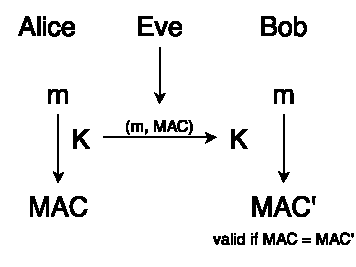
\includegraphics{images/2-sym-AB.pdf}
\end{center}

\textbf{Disadvantages:} key must be shared over secure channel, requires unique key for pairs of commuicating people.

\textbf{Advantages:} simple to use, fast computations

\subsection{Public-key authentication}
Signs with \emph{private} key, verifies with \emph{public} key (reverse of pub-key encryption/decryptions).

\begin{center}
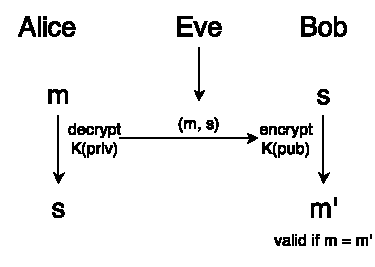
\includegraphics{images/2-pub-AB.pdf}
\end{center}

\textbf{Advantages:} no shared key (does not require secure channel to exchange keys), same public key can be used by everyone.

\textbf{Disadvantages:} existential forgery is trivial, Eve can choose any $s$ and compute corresponding $e_{pub}(s) = m$. Hash functions can solve this.

\subsection{RSA}

%%% Local Variables: 
%%% mode: latex
%%% TeX-master: "../index"
%%% End: 

\subsection*{Setup}
$H$ is a publicly known hash function, must be secure.

\textbf{Public key:} $(n, e)$ where $n = pq$ for primes $p, q$ and $e \in \mathbb{Z}_{\phi(n)}^*$

\textbf{Private key:} $(p, q, d)$ where $d \in \mathbb{Z}_{\phi(n)}^*$, such that
\[ ed \equiv 1 \mod \phi(n) \]

We use $\phi(n)$ because it is hard to compute given only $n$, but
easy with known $p, q$ since $\phi(n) = (p-1)(q-1)$, thus $d$ cannot
be easily computed given just $n$ (must prime factor $n$).

\textbf{Signature:} $m$ is the message and $x = H(m) \in \mathbb{Z}_n$. Signature is
\[ s = x^d \mod n \]

\textbf{Verification:} $m$ is the message, signature is $s \in \mathbb{Z}_n$. Accept if
\[ x \equiv s^e \mod n \]

\subsection{Hash-functions}
$H$ is used to prevent the trivial forgey where Eve can choose any $s$
such that $s = e_{pub}(m)$. She cannot do this since she would need a
preimage for $H(m)$ as $s$ otherwise does not sign $H(m)$ but $m$.



\subsubsection*{Proof}
%%% Local Variables:
%%% mode: latex
%%% TeX-master: "../index"
%%% End:

\textbf{Public:} $n = pq$ for primes $p, q$ and encryption exponent $e
\in \mathbb{Z}_{\phi(n)}^*$

\textbf{Private:} $(p, q, d)$ where $d \in \mathbb{Z}_{\phi(n)}^*$, such that
\[ ed \equiv 1 \mod \phi(n) \]

Define $\phi(n) = (p-1)(q-1)$. We have that
\begin{align*}
  & ed \equiv 1 \mod \phi(n)\\
  \Rightarrow\quad& ed = 1 + k(p - 1)(q - 1) \quad \text{where } k \in \mathbb{Z}
\end{align*}

We need to prove that $(m^e)^d \equiv m \mod$ since that is enc and dec using RSA.
\begin{align*}
(m^e)^d &\equiv m \mod n \\
\Rightarrow\quad m^{ed} &\equiv m \mod n
\end{align*}

Chinese remainder says that it is enough to show
\[ m^{ed} \equiv m \mod p \textbf{ and } m^{ed} \equiv m \mod q \]

Showing for $p$. There are two cases: 1) $m \equiv 0 \mod p$ and 2) $m \not\equiv 0 \mod p$.

\textbf{Case 1}
\begin{align*}
m &\equiv 0 \mod p\\
\Rightarrow\quad m^x &\equiv m \mod p \quad \text{where } x \in \mathbb{Z}
\end{align*}
and since $ed \in \mathbb{Z}$ case 1 holds.

\textbf{Case 2}
\begin{align*}
m^{ed} &\equiv m \mod p\\
m^{1 + k(p-1)(q-1)} &\equiv m \mod p\\
m \cdot m^{k(p-1)(q-1)} &\equiv m \mod p\\
m \cdot (m^{(p-1)})^{k(q-1)} &\equiv m \mod p
\end{align*}

From \textbf{Fermats little theorem} (\ref{sec:fermats-little}) we
know that $x^{p-1} \equiv x \mod p$ for prime $p$. Thus
\begin{align*}
m \cdot 1^{k(q-1)} &\equiv m \mod p\\
m \cdot 1 &\equiv m \mod p\\
m &\equiv m \mod p
\end{align*}

Therefore, case 2 also holds and we have proved for prime $p$.
